%!TEX program = xelatex
\documentclass{beamer}
\usepackage[backend=biber,style=numeric-comp,sorting=none]{biblatex}
\addbibresource{biblio.bib}

\usecolortheme[light,accent=orange]{solarized}

\usepackage{subcaption}
\usepackage{gitdags}

\usepackage{blindtext}
\usepackage{xltxtra}
\usepackage{wrapfig}

\usepackage{listings}
\usepackage{multicol}
\usepackage{verbatim}

\defaultfontfeatures{Ligatures=TeX}

\title{Oh my GIT!}
\subtitle{Git ate my work and other stories}
\author{Vojtěch Vladyka}
\date{31.8.2019}

% \setbeamercolor
%
% solarizedBase03
% solarizedBase02
% solarizedBase01
% solarizedBase00
% solarizedBase0
% solarizedBase1
% solarizedBase2
% solarizedBase3
% solarizedYellow
% solarizedOrange
% solarizedRed
% solarizedMagenta
% solarizedViolet
% solarizedBlue
% solarizedCyan
% solarizedGreen

\begin{document}
    \frame{\titlepage}
    \begin{frame}
       \frametitle{Table of contents}
       \begin{enumerate}
           \item What is git
           \\   \textcolor{solarizedRebase01}{\footnotesize\hspace{1em} ...and why you should care}	
           \item Setup git
           \\   \textcolor{solarizedRebase01}{\footnotesize\hspace{1em} Clients, differences, common issues}	
           \item Git vs. SVN
           \\   \textcolor{solarizedRebase01}{\footnotesize\hspace{1em} King is dead, long live the King!}	
           \item Git essentials
           \\   \textcolor{solarizedRebase01}{\footnotesize\hspace{1em} Git controls crash course}	
           \item Scenarios
           \\   \textcolor{solarizedRebase01}{\footnotesize\hspace{1em} We are going to break things there. A lot.}	
           \item QA
           \\   \textcolor{solarizedRebase01}{\footnotesize\hspace{1em} Umm, why was I here again?}
       \end{enumerate}
    \end{frame}
    \section{What is git?}
    \begin{frame}
        \frametitle{What is git?}
        \begin{itemize}
            \item version control system made by Linus Torvalds (mostly) at 2005 for Linux Kernel development
            \item always capture state of working tree
            \item focused on distributed development
            \item supports rapid branching \& merging
            \item it is pronounced GIT with G like GIF ~\footfullcite{linus-speech}
        \end{itemize}
    \end{frame}
    \begin{frame}
        \frametitle{Differences between Git and SVN}
        \begin{itemize}
            \item Git is distributed by design
            \item Works with whole sourcetree (unlike SVN which works with individual files and their revisions)
            \item Strong support for non-linear development $\rightarrow$ rapid branching \& merging
            \item Cryptographic authentication of history - every commit has SHA-1 hash of everything leading to that point
        \end{itemize}
    \end{frame}
    \begin{comment}
    \begin{frame}
        \begin{tikzpicture}
            % Commit DAG
            \gitDAG[grow right sep = 2em]{
                A -- B -- {
                  C,
                  D -- E,
                }
            };
            % Tag reference
            \gittag
                [v0p1]      % node name
                {v0.1}      % node text
                {above=of A}% node placement
                {A}         % target
            % Remote branch
            \gitremotebranch
                [originmaster]
                {origin/master}
                {above=of C}
                {C}
            % Branch
            \gitbranch
                {master}
                {above=of E}
                {E}
            % HEAD reference
            \gitHEAD
                {above=of master}
                {master}
        \end{tikzpicture}
    \end{frame}
    \end{comment}
    \begin{frame}[fragile]
        \frametitle{Git essentials}
        \begin{multicols}{2}
        \begin{lstlisting}[gobble=12]
            git init                
                clone

                fetch
                merge
                push
                pull

                branch
                checkout
                merge
                branch -d
        \end{lstlisting}
        \begin{lstlisting}[gobble=12]
            git log                
                log --follow [file]

                add
                commit

                reset
                reset --hard
                stash

                rebase
                cherrypick
                squash
        \end{lstlisting}
        \end{multicols}
    \end{frame}
    \begin{frame}
        \frametitle{Git essentials}
        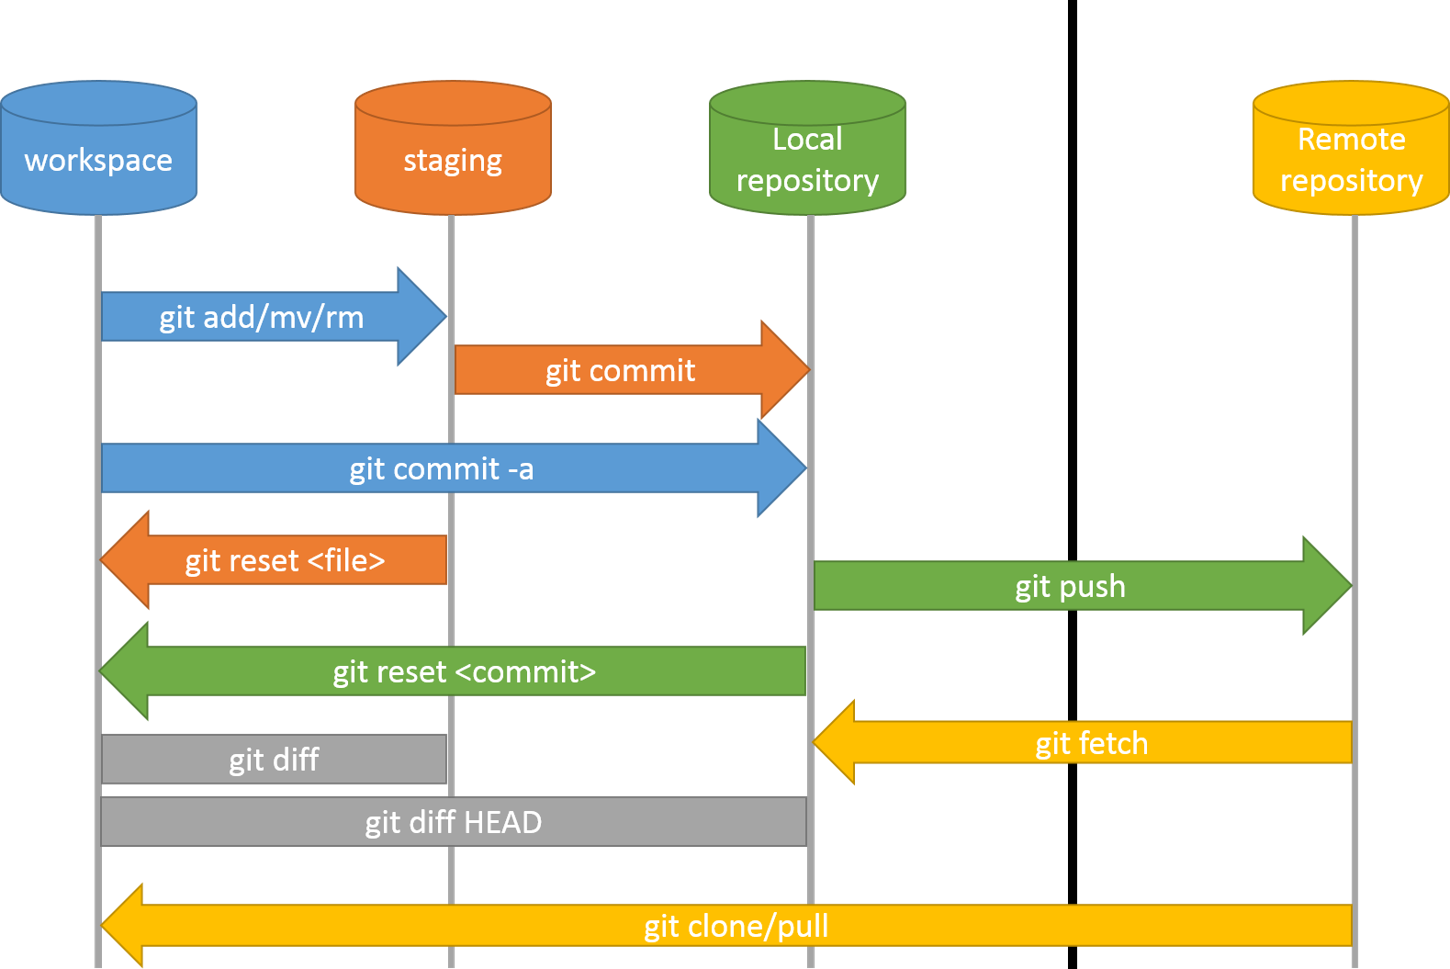
\includegraphics[width=\textwidth]{workflow.png}
    \end{frame}
    \begin{frame}[fragile]
        \frametitle{Git essentials}
        \begin{lstlisting}[gobble=12]
            $ git init
        \end{lstlisting}
        $\rightarrow$ initialize new repository in current directory with all its contents
        \begin{lstlisting}[gobble=12]
            $ git clone https://somerepo.com/repo.git
        \end{lstlisting}
        $\rightarrow$ downloads repository with all current branches \& commits
    \end{frame}
    \begin{frame}[fragile]
        \frametitle{Git essentials}
        \begin{lstlisting}[gobble=12]
            $ git checkout -b feature1
            $ (git branch feature1 ; git checkout feature1)
        \end{lstlisting}
        \begin{tikzpicture}
            % Commit DAG
            \gitDAG[grow right sep = 2em]{
                A -- B -- C -- {
                    D,
                    E -- F
                }
            };
            % Branch
            \gitbranch
                {master}
                {above=of D}
                {D}
            % Branch
            \gitbranch
                {feature1}
                {above=of F}
                {F}
            % HEAD reference
            \gitHEAD
                {above=of feature1}
                {feature1}
        \end{tikzpicture}
        \begin{lstlisting}[gobble=12]
            $ git checkout master
            $ git merge feature1
        \end{lstlisting}
        \begin{tikzpicture}
            % Commit DAG
            \gitDAG[grow right sep = 2em]{
                A -- B -- C -- {
                    D,
                    E -- F
                } -- G
            };
            % Branch
            \gitbranch
                {master}
                {below=of G}
                {G}
            % Branch
            \gitbranch
                {feature1}
                {below=of F}
                {F}
            % HEAD reference
            \gitHEAD
                {below=of master}
                {master}
        \end{tikzpicture}

    \end{frame}
    \begin{frame}[fragile]
        \frametitle{Git essentials}
        \begin{lstlisting}[gobble=12]
            git log
            git ....
            git log --follow [file]
        \end{lstlisting}
    \end{frame}
    \begin{frame}[fragile]
        \frametitle{Git essentials}
        \begin{lstlisting}[gobble=12]
            git stash
            git stash push
            git stash pop
            git stash apply stash@{2}
            git checkout stash@{2} -- somefile
        \end{lstlisting}
    \end{frame}
    \begin{frame}
        \frametitle{Dotazy?}
    \end{frame}
    \section{Děkujeme za pozornost}
\end{document}
